In het volgende hoofdstuk is zijn de lasten van de moonrover bepaald. Op basis van deze gegevens kunen we de juiste motor gaan selecteren voor de moonrover. Door de leverancier "Maxon" is er een advies gedaan van een reeks motoren en transmissies;
\begin{align*}
        motor: &RE25 1187xx\\
        transmissie: &Planetary Gearhead GP xx xx
\end{align*}
In dit hoofdstuk zullen wij een keuze gaan maken voor een specifieke motor in combinatie met een specifieke transmissie.


\subsection{Motorkeuze}
Binnen de aangegeven maxon reeks hebben wij gekozen voor de RE25 118745. In theorie is het mogelijk om elke motor te kieze binnen de aangegeven reeks in combinatie met de juiste transmissie. Voor deze specifieke situatie hebben we gekozen voor de RE25 118745. Dit is een wat kleinere motor binnen de reeks, echter is het mooie van deze motor dat hij een efficiëntie van 90\% heeft. In afbeelding \ref{fig:RE25_118745} is te zien hoe de koppel toeren karakteristiek van de motor zich weerhoud tegen de last. In combinatie met de juiste transmissie kan deze motor goed ingezet worden bij de moonrover. In Bijlage \ref{app:datasheet motor} is de datasheet te zien van deze motor.
        \begin{figure}[H]
                \centering
                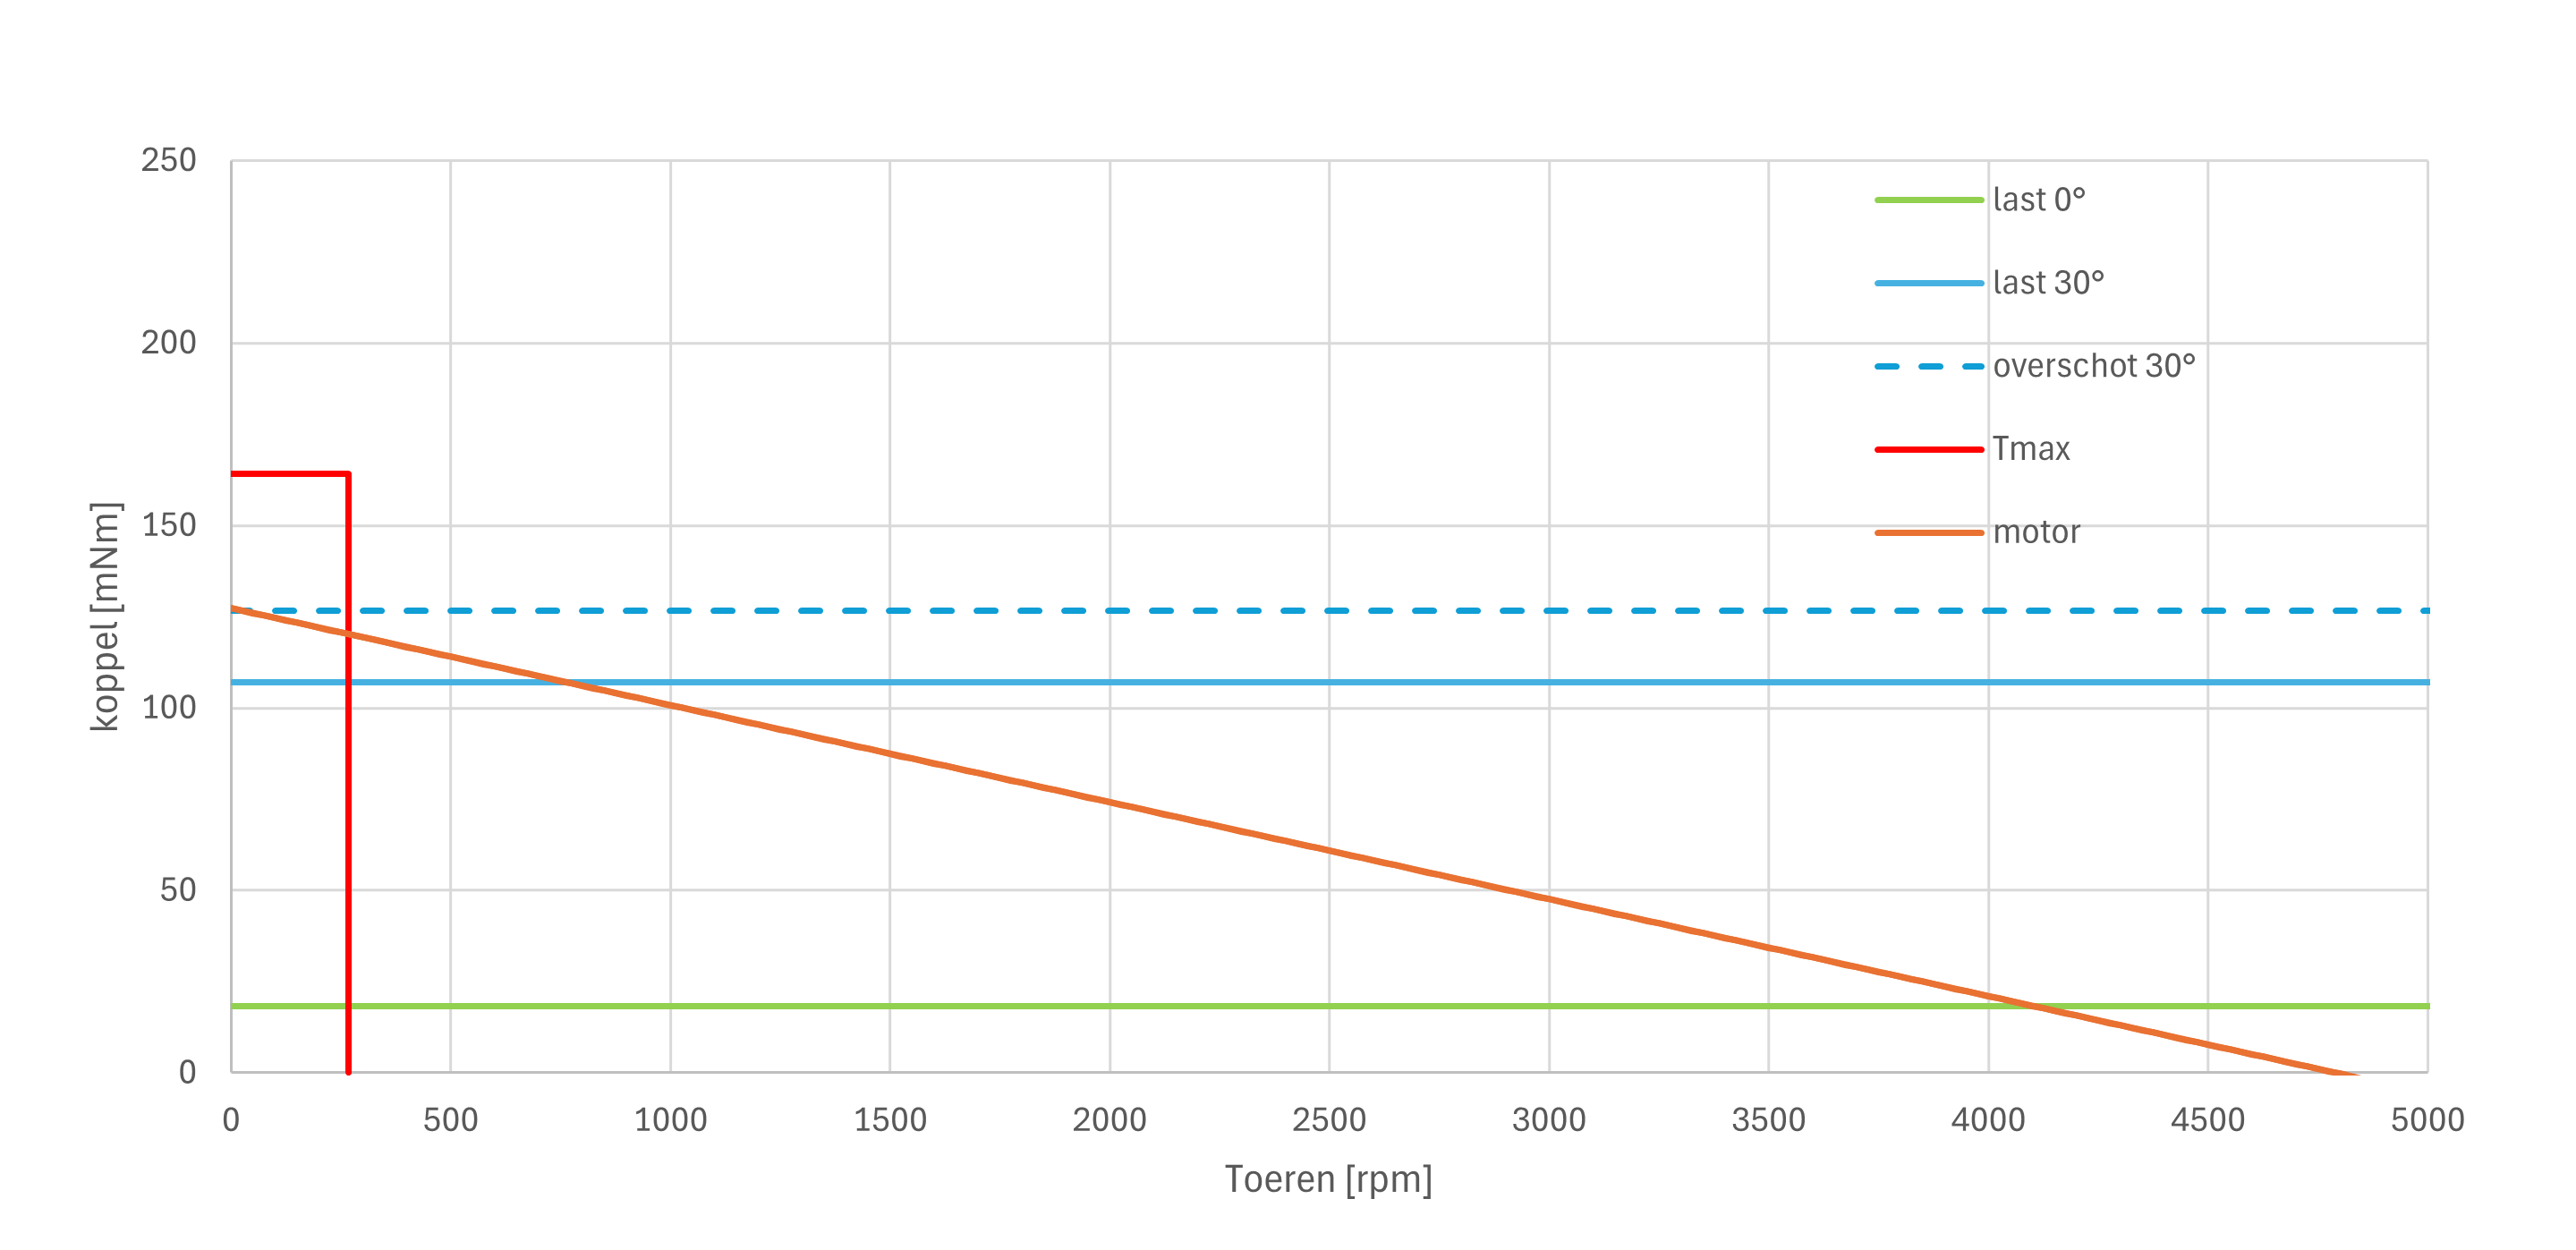
\includegraphics[scale=0.7]{RE25_118745.png}
                \caption{koppel toeren karakteristiek RE25 118745}
                \label{fig:RE25_118745}
        \end{figure}

\newpage

\subsection{transmissiekeuze}
In afbeelding \ref{fig:RE25_118745} is duidelijk te zien dat een transmissie duidelijk aan te raden is voor het gebruiken van deze motor in de situatie van de moonrover. Het maximale koppel is eignelijk aan de lage kant en zonder transmissie maakt de motor veel ste veel toeren. Door gebruik te maken van een transmissie kunnen we er voor zorgen dat er meer koppel beschikbaar komt met minder toeren. Hierdoor zal de motor efficiënten gaan Werken omdat hij minder torque hoeft te leveren en hij vaker rond zijn nominale toerental zal draaien. In de datasheet van de  motor (bijlage \ref{app:datasheet motor}) worden er voor deze motor een aantal transmissies aangeraden binnen deze selectie en de selectie van maxon hebben wij gekozen voor de Planetary Gearhead GP 32 A 166158. Deze transmissie heeft een gear ratio van 14:1 en een efficitie van 75\%. Met deze eigenschappen zal de koppel toeren karakteristiek veranderen wat te zien is in afbeelding \ref{fig:GP 32 A 166158} hier is duidelijk te zien dat met deze transmissie de de wielen niet veel te hard kunnen draaien en dat er meer dan voldoende torque beschikbaar is voor de moonrover. Het extra koppeloverschot zorgt er ook nog voor dat de motor niet te hard hoeft te werken om de moonrover te kunnen verplaatsen.

        \begin{figure}[H]
                \centering
                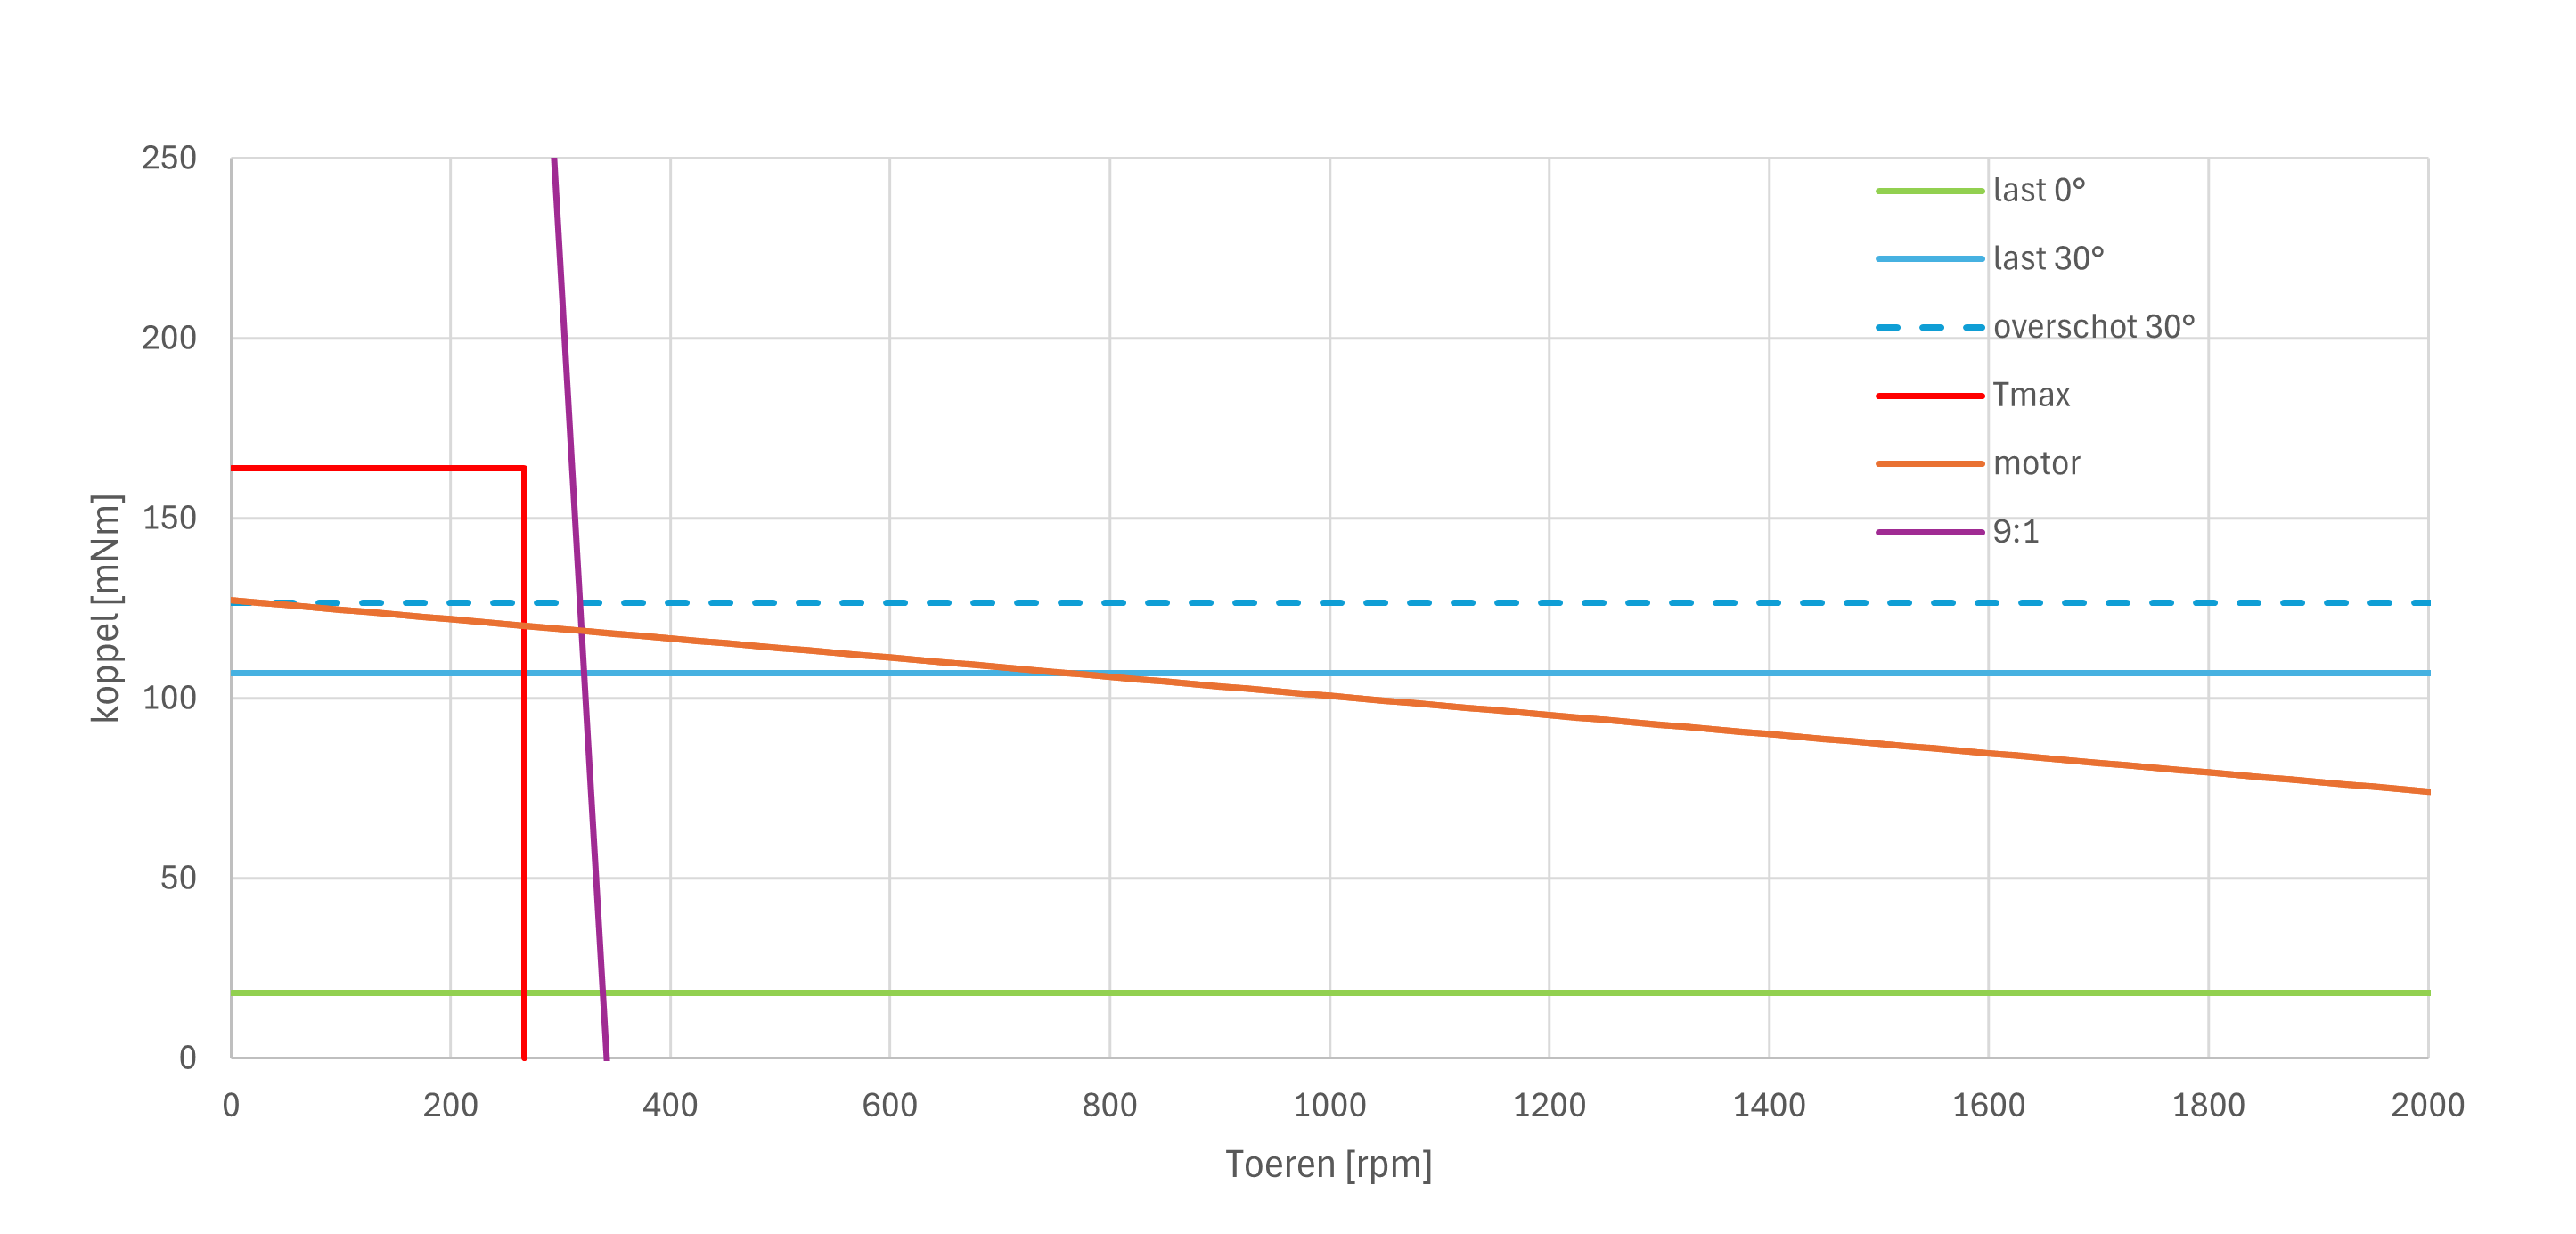
\includegraphics[scale=0.7]{GP_32_A_166158.png}
                \caption{koppel toeren karakteristiek met GP 32 A 166158}
                \label{fig:GP 32 A 166158}
        \end{figure}

\subsection{efficiëntie}

Hier onder word het vermogen berkend wat de motor opneemt bij een bepaalde hoeveelheid koppel. In afbeelding \ref{fig:vermogenskarakteristiek} te zien hoe het minimale en maximale vermogen zich weerhoud tegen de helling waar de moonrover op rijdt. Dit is het vermogen wat in de motor gaat.

\begin{multicols}{2}
        \textbf{Formules:}
        \begin{equation}
            \begin{split}
                P &= F \cdot v \\
                F &= \frac{T}{r} \\
                &\Downarrow \\
                P &= 5.25 [W]
            \end{split}
        \end{equation}

        \textbf{constante:}
        \begin{equation*}
            \begin{split}
                v &= 2.1 [m/s] \\
                T &= 0.1265[mNm]  \\
                r &= 0.075[m]
            \end{split}
        \end{equation*}
    \end{multicols}

    \begin{figure}[H]
        \centering
        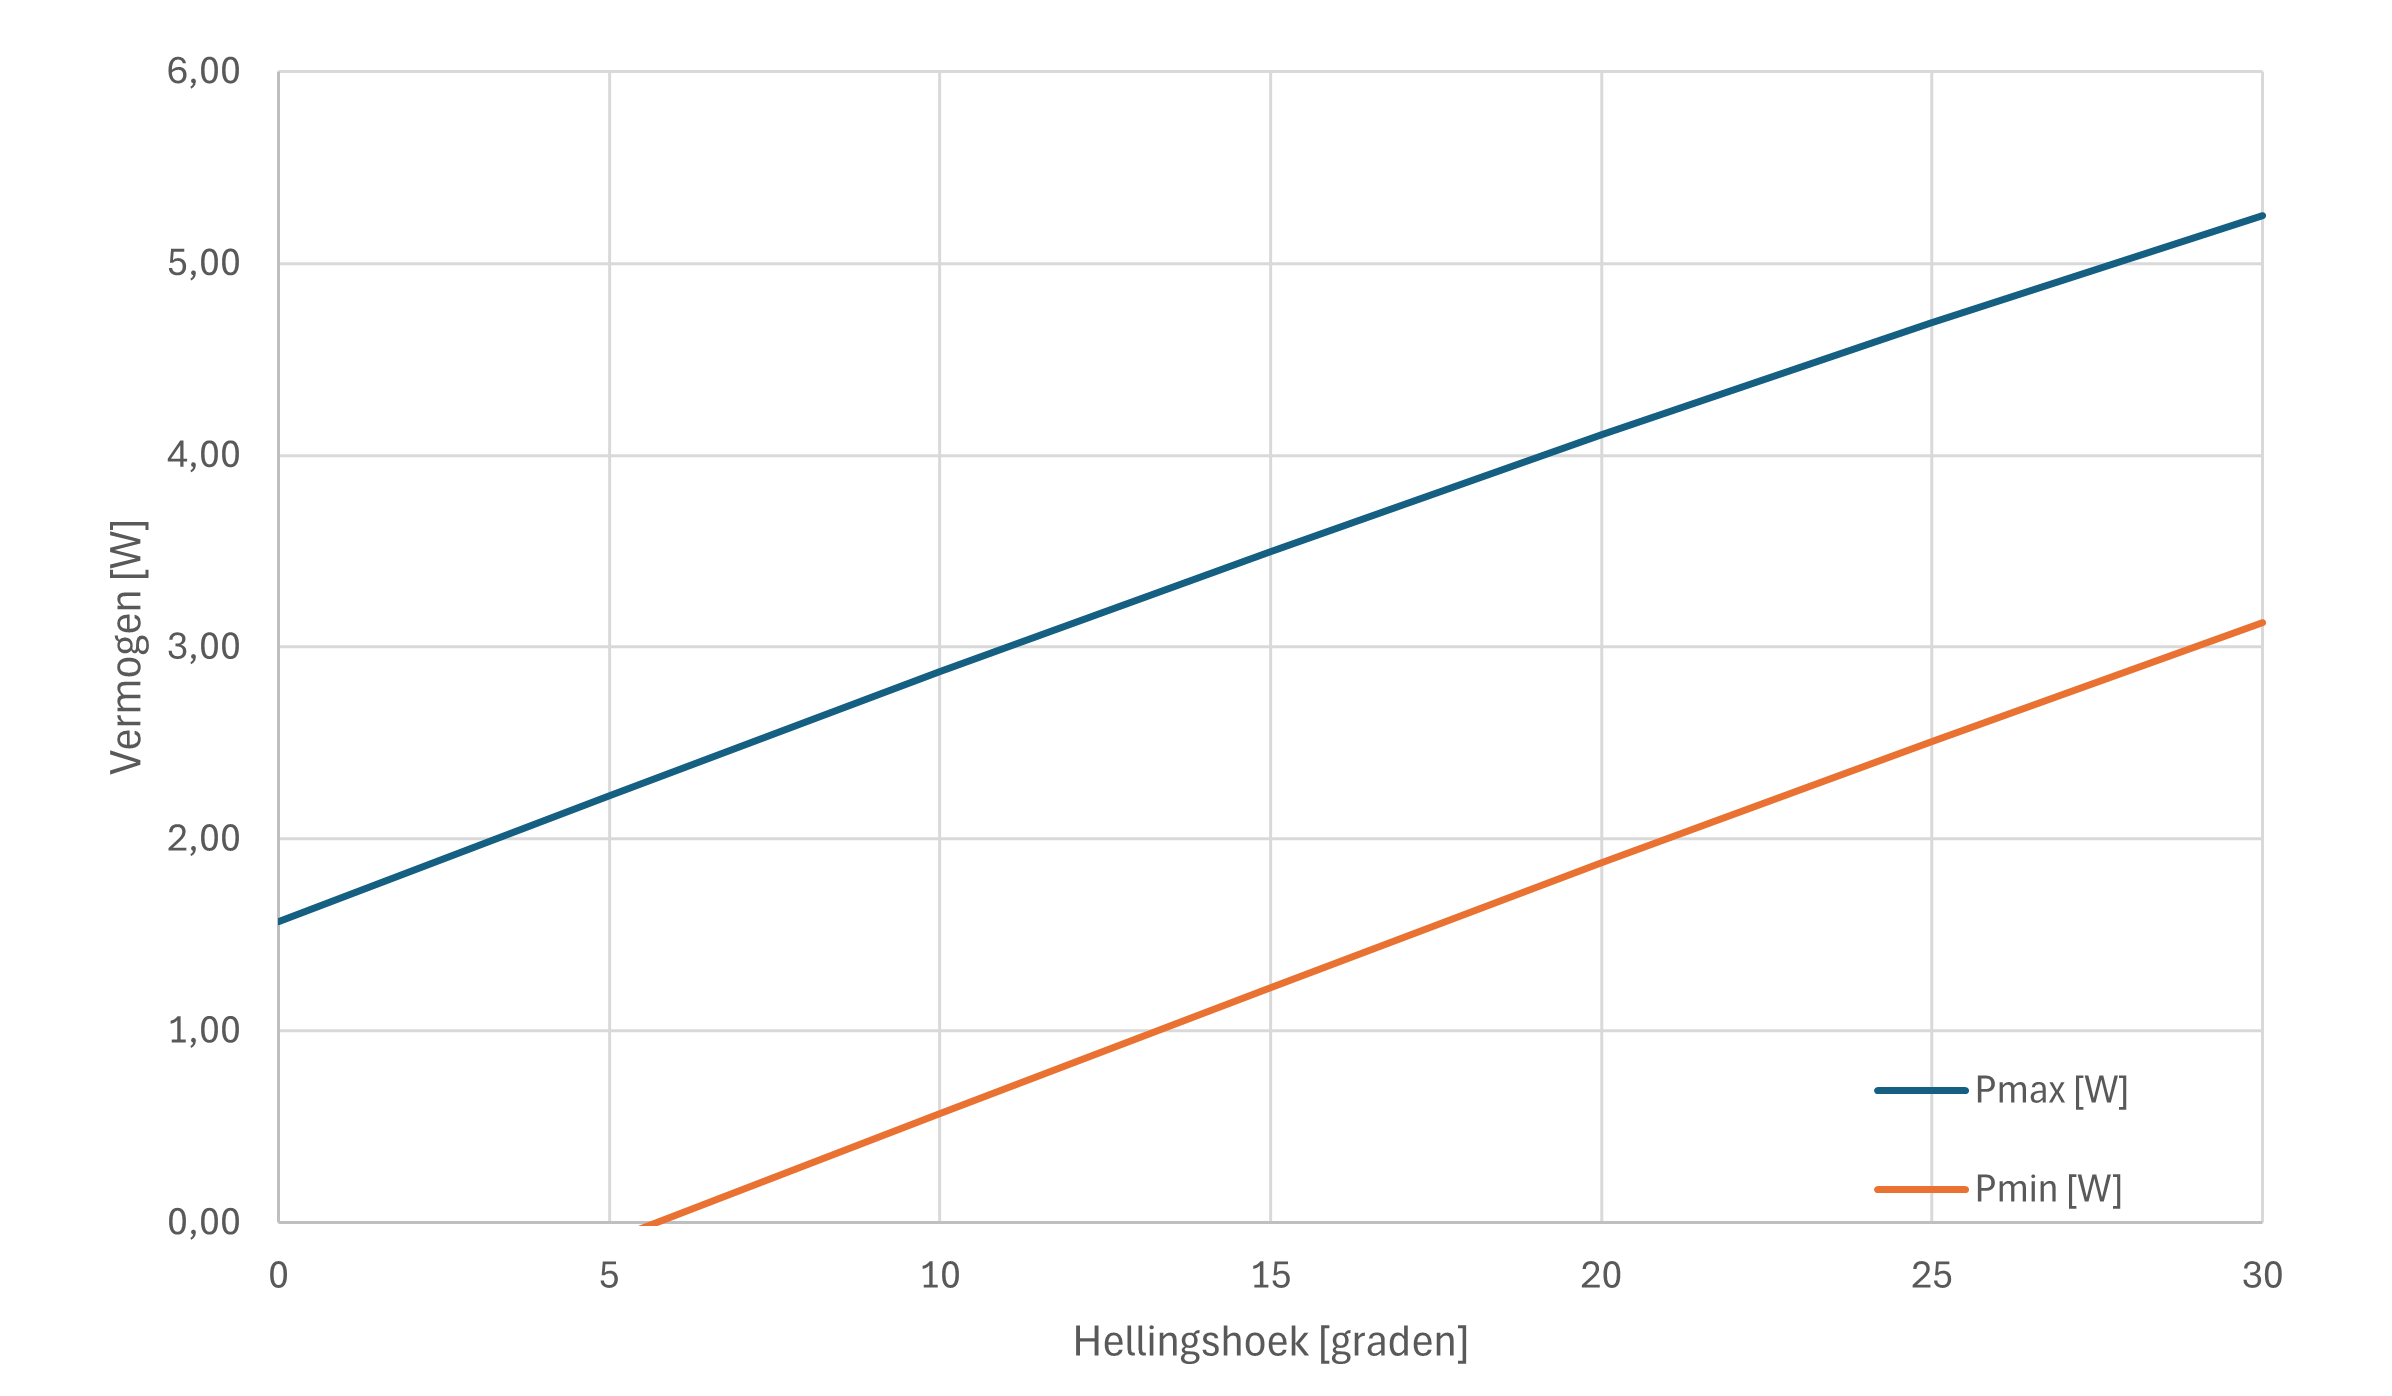
\includegraphics[scale=0.7]{vermogenskarakteristiek.png}
        \caption{vermogenskarakteristiek}
        \label{fig:vermogenskarakteristiek}
        \end{figure}

De motor heeft een efficiëntie van een 90\%

De transmissie heeft een efficiëntie van 75\%

Samen komt dit op een totaal efficiëntie van 67,5\% \\
Dit betekent dat er van het vermogen wat er in de motor gaat er 67,5\% effectief gebruikt word en de rest opgaat in warmte etc.

\subsection{Warmtedisipatie}

Voor de moonrover zullen de motoren geleverd worden van het merk Maxon. Maxon heeft aangegeven dat zij de gekozen motor "maan bestendig" zullen maken. Hierbij zal ook rekening gehouden met de temperatuur verschillen op de maan en de warmte dissipatie hiervan. 